\documentclass{article}
\usepackage[section]{placeins}
\usepackage{graphicx}

\author{Yaghoub Shahmari}
\title{Report - Problem Set no 1}
\date{\today}
\graphicspath{ {../Figs/} }

\begin{document}
    \maketitle
    \section*{Problem 1}
    \textbf{Basic description:}

    There we want to simulate the Koch curve using computational methods.
    In that case, we have to follow the algorithm which leads us to the solution.
    At first, we have a list of 2 points that create a single line.
    Then we have to create three more points between them and transmit them to the position they have to go.
    At first, we divide the line into third.
    Add the final point of the line in the middle of our list.
    Then we will do that again but we will divide the first line to two-thirds instead of third.
    Then we will rotate the final spot in 60 degrees and add the point before the last point in the list.
    And finally, we will do the previous operation without rotation.
    We have to repeat these operations for every point side by side in the initial list (the initial list in every step will be updated and will contain more points).

    I implemented the algorithm for the few shapes, apart from the line,
    I also applied the algorithm in some triangles
    (the rotation degrees for them were 60, -60, and 120).
    The results are as follows:

    \begin{figure}[!htb]
        \centering
        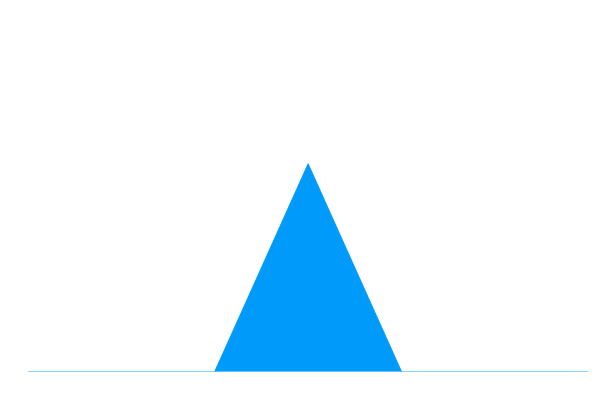
\includegraphics[scale = 0.15]{/Q1/KochCurve1O1}
        \label{fig:1.1.1}
        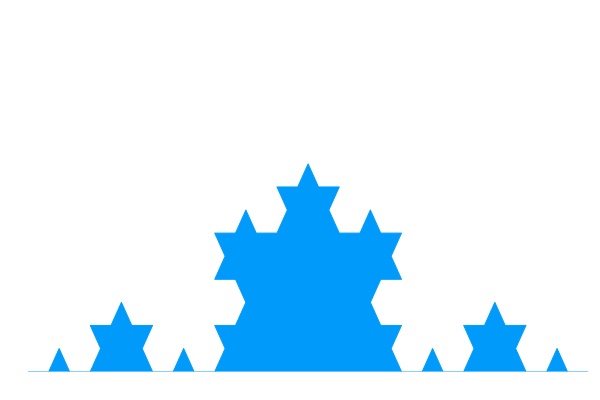
\includegraphics[scale = 0.15]{/Q1/KochCurve1O2}
        \label{fig:1.1.2}
        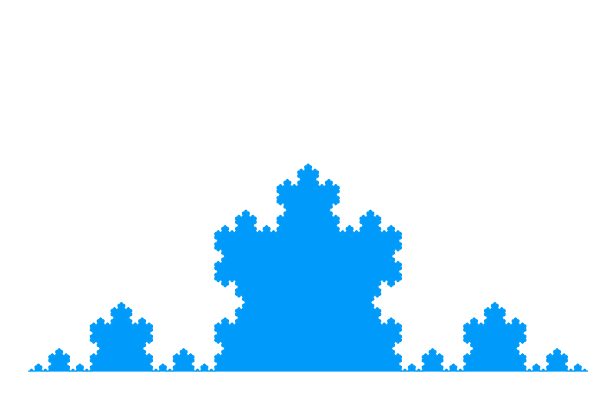
\includegraphics[scale = 0.15]{/Q1/KochCurve1O5}
        \label{fig:1.1.3}
        \caption{Koch curve for a single line. The figures belong to the first, second, and fifth stages, respectively.}
    \end{figure}
    \begin{figure}[!htb]
        \centering
        
\includegraphics[scale = 0.15]{/Q1/KochCurve2O1}
        \label{fig:1.2.1}
        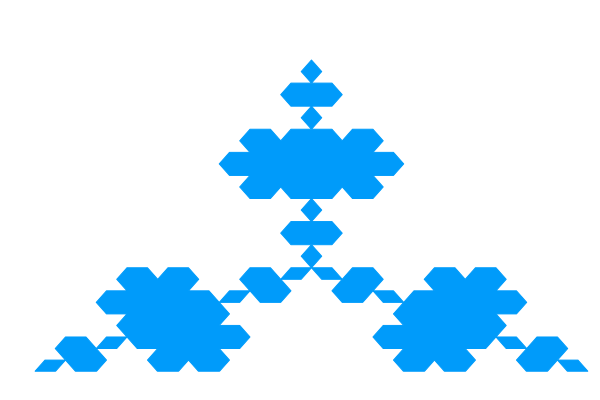
\includegraphics[scale = 0.15]{/Q1/KochCurve2O2}
        \label{fig:1.2.2}
        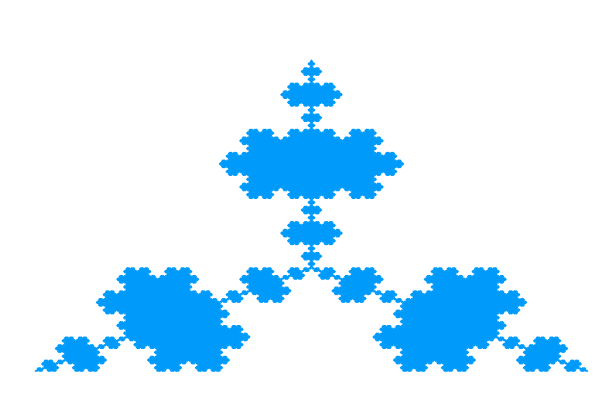
\includegraphics[scale = 0.15]{/Q1/KochCurve2O5}
        \label{fig:1.2.3}
        
\includegraphics[scale = 0.15]{/Q1/KochCurve3O1}
        \label{fig:1.3.1}
        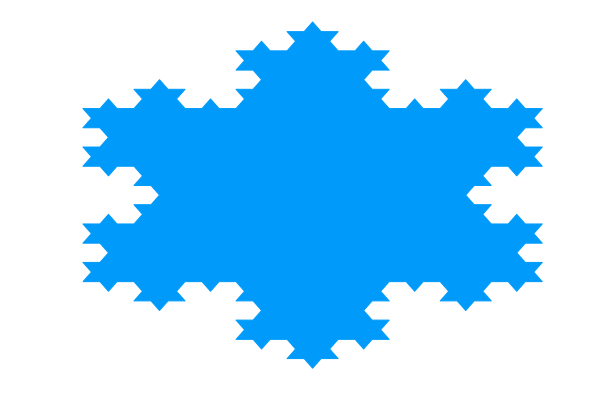
\includegraphics[scale = 0.15]{/Q1/KochCurve3O2}
        \label{fig:1.3.2}
        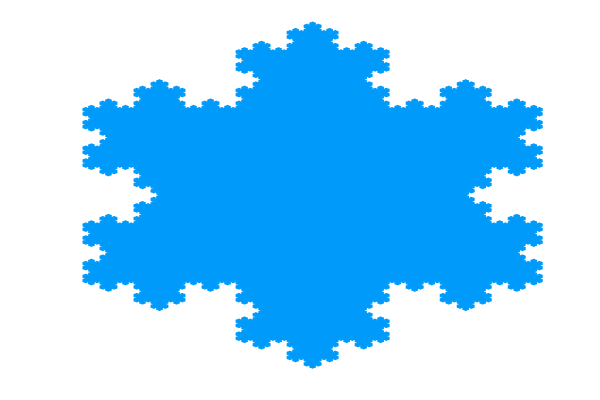
\includegraphics[scale = 0.15]{/Q1/KochCurve3O5}
        \label{fig:1.3.3}
        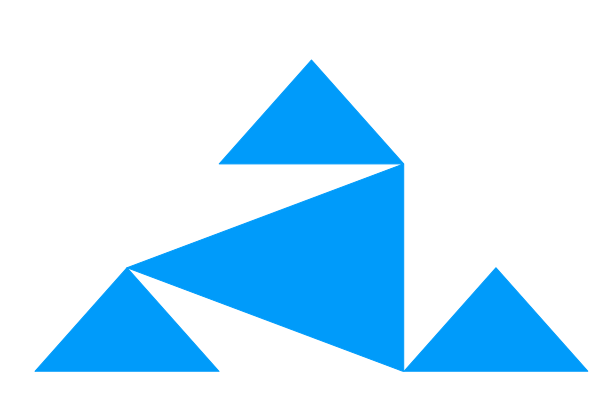
\includegraphics[scale = 0.15]{/Q1/KochCurve4O1}
        \label{fig:1.4.1}
        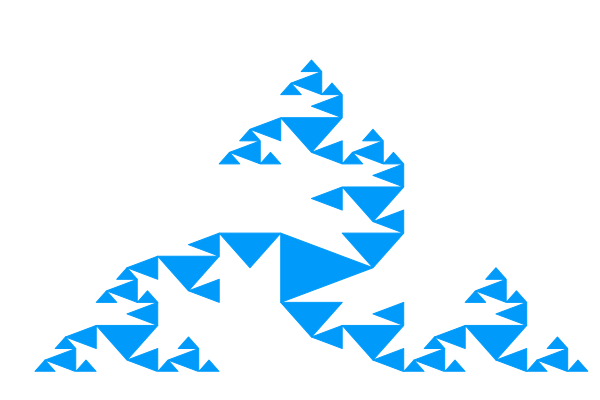
\includegraphics[scale = 0.15]{/Q1/KochCurve4O2}
        \label{fig:1.4.2}
        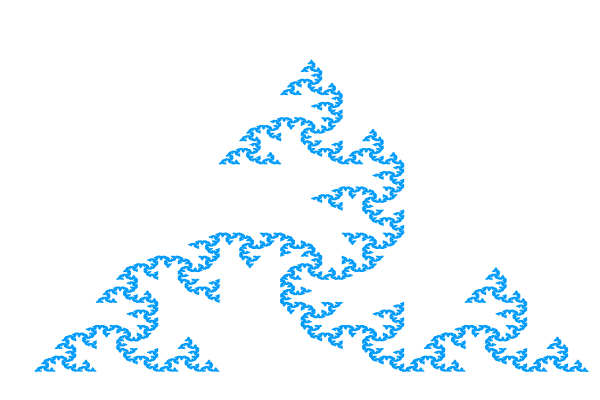
\includegraphics[scale = 0.15]{/Q1/KochCurve4O5}
        \label{fig:1.4.3}
        \caption{Koch curve for triangles (The rotation degrees are 60, -60, and 120 respectively, from up to down). The figures belong to the first, second, and fifth stages, respectively.}
    \end{figure}

    \section*{Problem 2}
    \textbf{Basic description:}

    There we want to simulate the Heiway dragon using computational methods.
    As before we have to transmit and rotate our points to create what we want.
    We must note that our rotation degree is 45 degrees.
    We have to rotate the whole structure one by one with 45 and -45 degrees.
    However, if we change both rotation degrees to -45 we will have the Lévy C curve.
    The results are as follows:
    \begin{figure}[!htb]
        \centering
        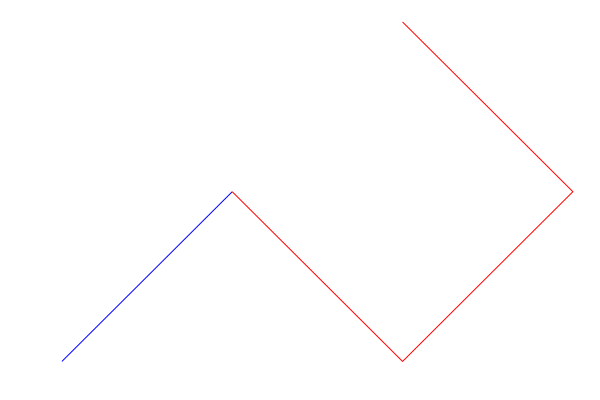
\includegraphics[scale = 0.13]{/Q2/Heighway-dragon-O1}
        \label{fig:2.1.1}
        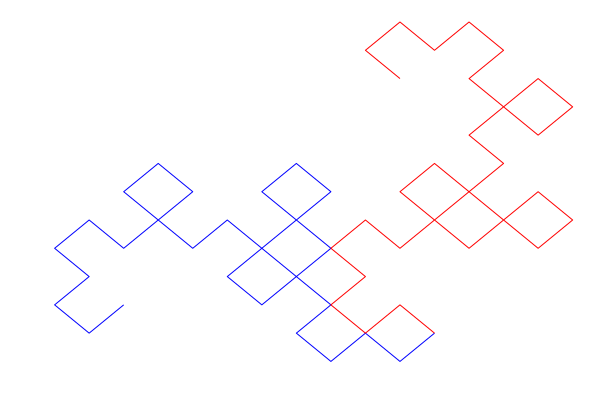
\includegraphics[scale = 0.13]{/Q2/Heighway-dragon-O5}
        \label{fig:2.1.2}
        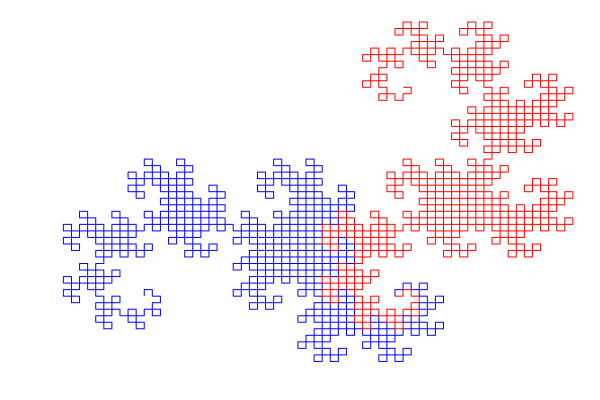
\includegraphics[scale = 0.13]{/Q2/Heighway-dragon-O10}
        \label{fig:2.1.3}
        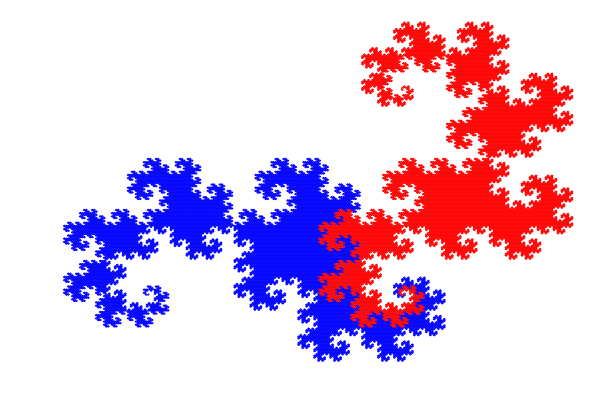
\includegraphics[scale = 0.13]{/Q2/Heighway-dragon-O15}
        \label{fig:2.1.3}
        \caption{The Heighway dragon fractal. The figures belong to the 1st, 5th, 10th, and 15th stages, respectively.}
    \end{figure}
    \begin{figure}[!htb]
        \centering
        \includegraphics[scale = 0.13]{/Q2/Lévy-C-curve-O1}
        \label{fig:2.2.1}
        \includegraphics[scale = 0.13]{/Q2/Lévy-C-curve-O5}
        \label{fig:2.2.2}
        \includegraphics[scale = 0.13]{/Q2/Lévy-C-curve-O10}
        \label{fig:2.2.3}
        \includegraphics[scale = 0.13]{/Q2/Lévy-C-curve-O15}
        \label{fig:2.2.3}
        \caption{The Lévy C curve fractal. The figures belong to the 1st, 5th, 10th, and 15th stages, respectively.}
    \end{figure}
    \section*{Problem 3}
    \textbf{Basic description:}

    There we want to simulate the Sierpinski triangle using computational methods.
    In that case, we must define a list of triangles that initially have only one triangle.
    In each step of our algorithm, the list will be updated and will contain more triangles.
    So we have to apply an algorithm that takes a single triangle from the list,
    makes it in four smaller triangles, and returns three of them (the center one won't return).
    You have to define a triangle as a list of the points that
make up our triangle
    And the coordinates of the points have to be divided in half.
    That would be enough for the first triangle but the others still need a transmission.
    And after all of our operations, a single triangle changed to three.
    we have to repeat these operations for every single triangle we have at the beginning of each stage.
    The results are as follows:
    \begin{figure}[!htb]
        \centering
        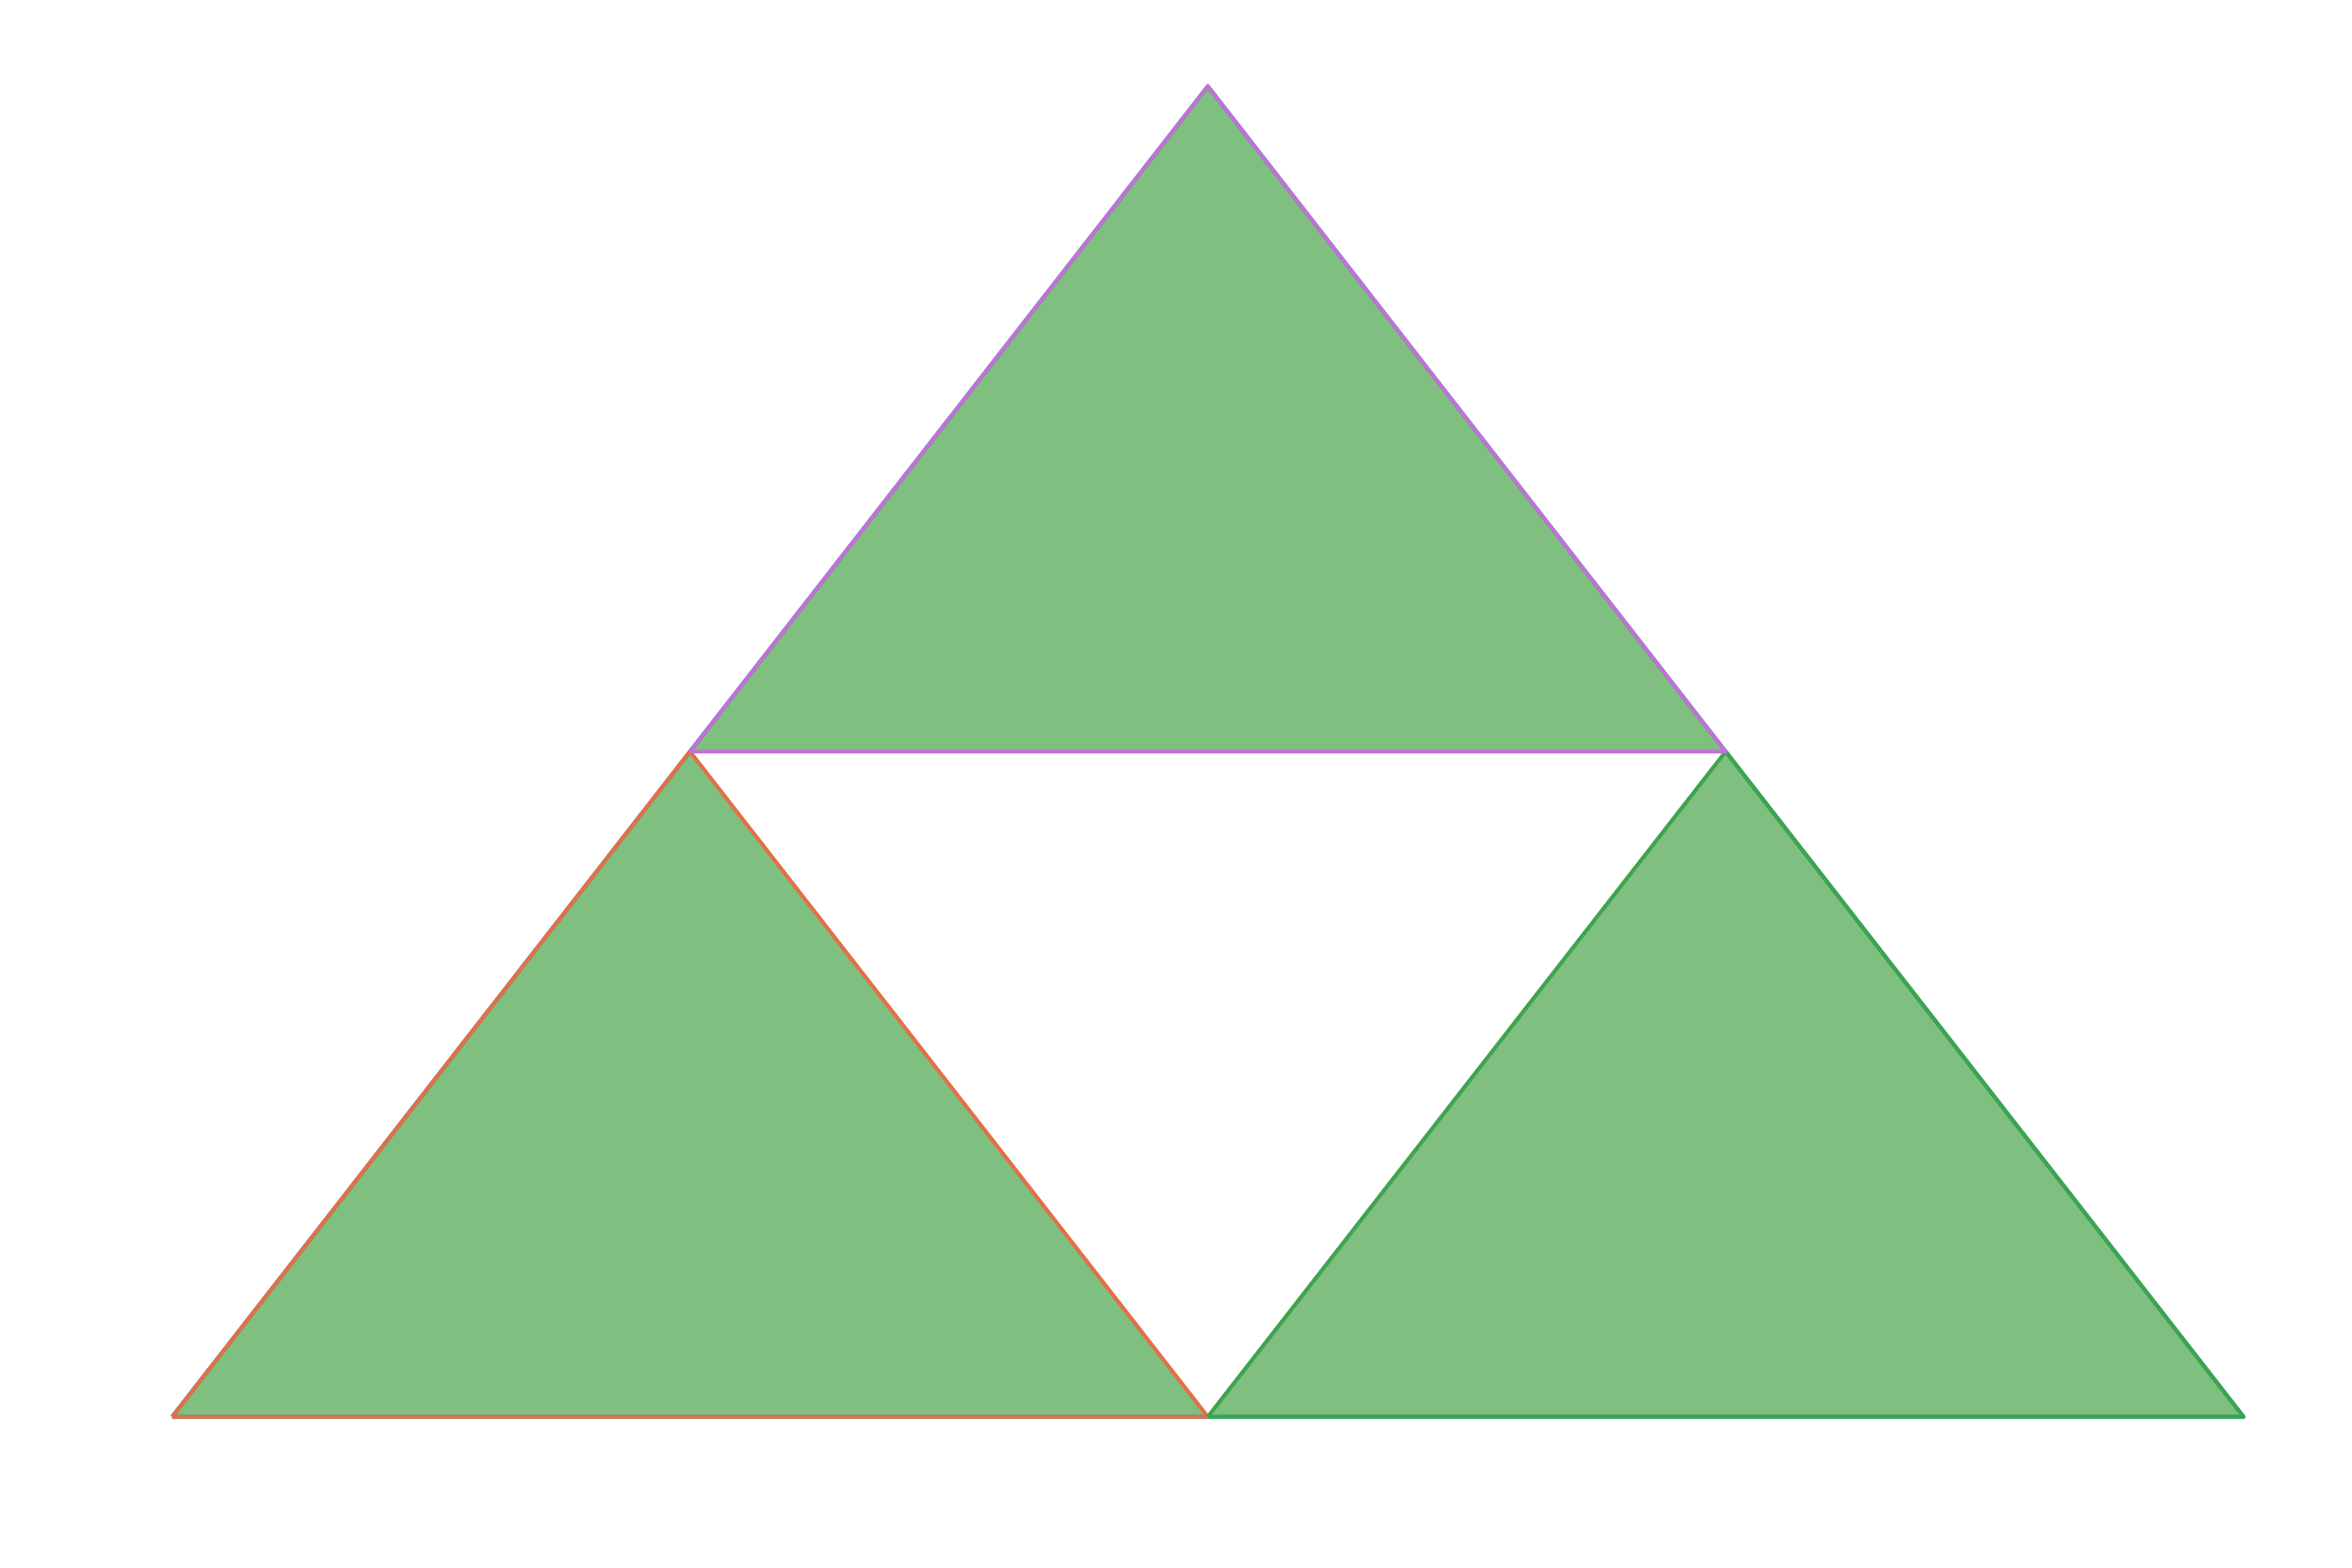
\includegraphics[scale = 0.027]{/Q3/SPT-O1}
        \label{fig:3.1.1}
        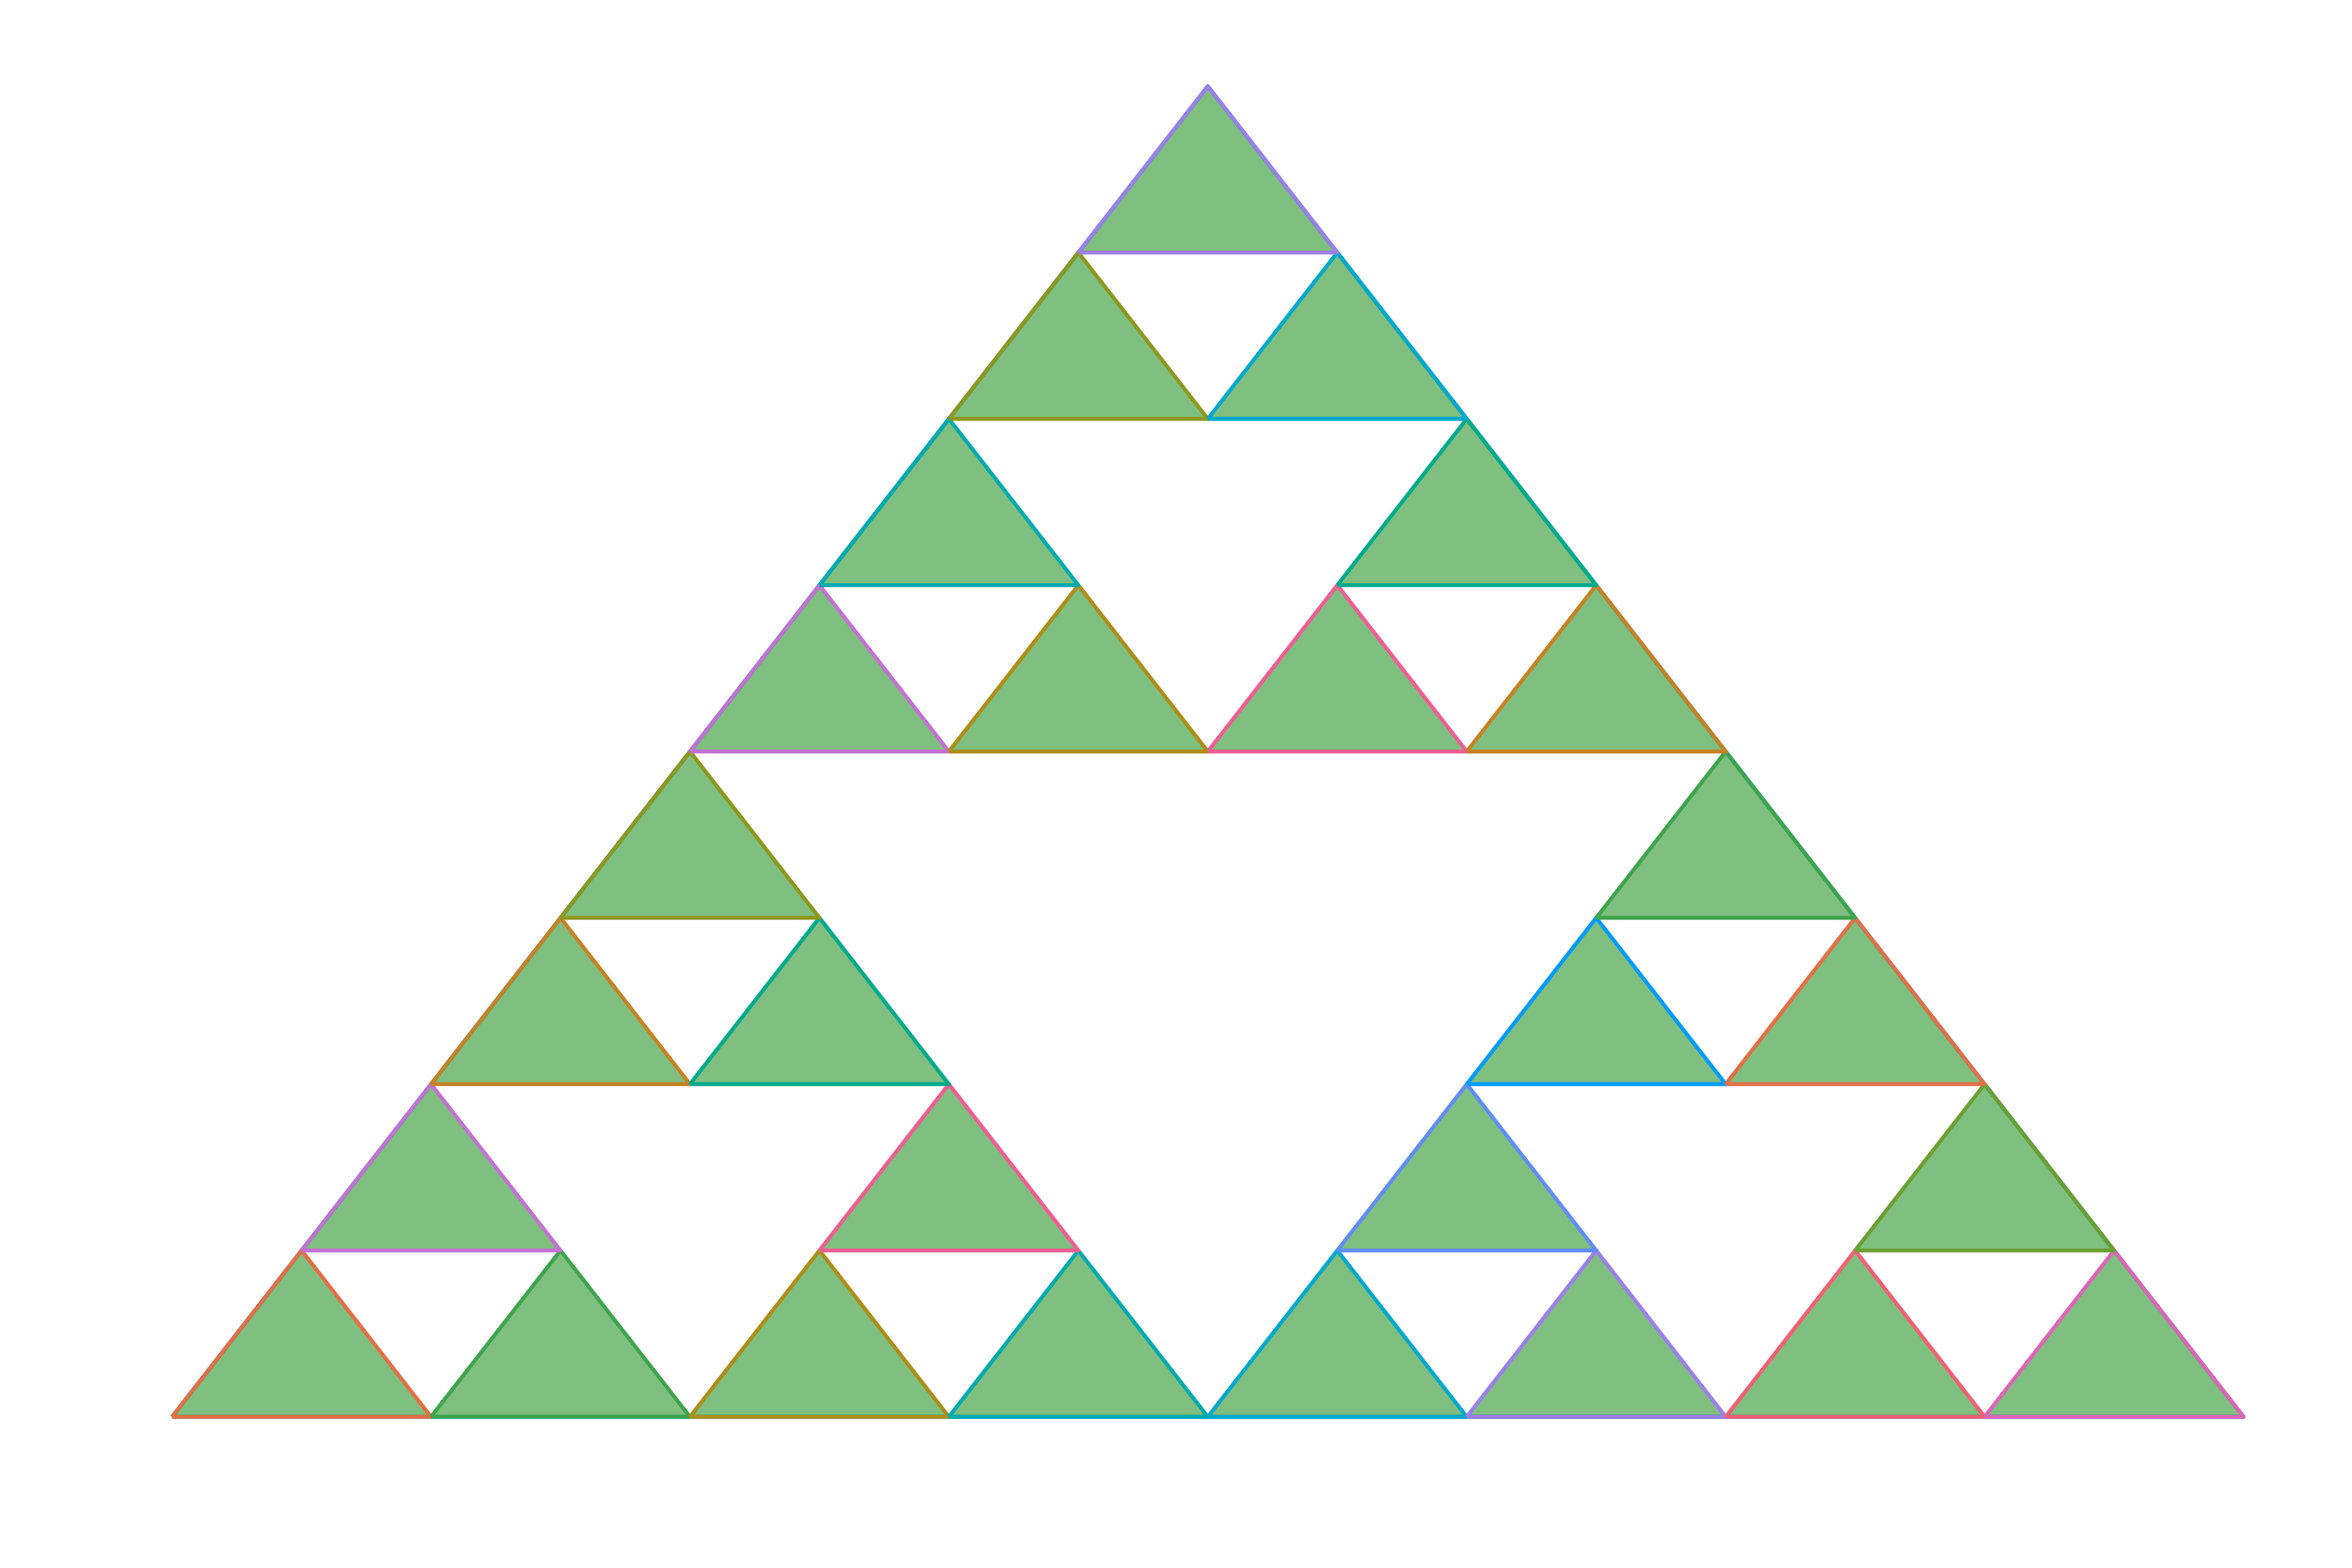
\includegraphics[scale = 0.027]{/Q3/SPT-O3}
        \label{fig:3.1.2}
        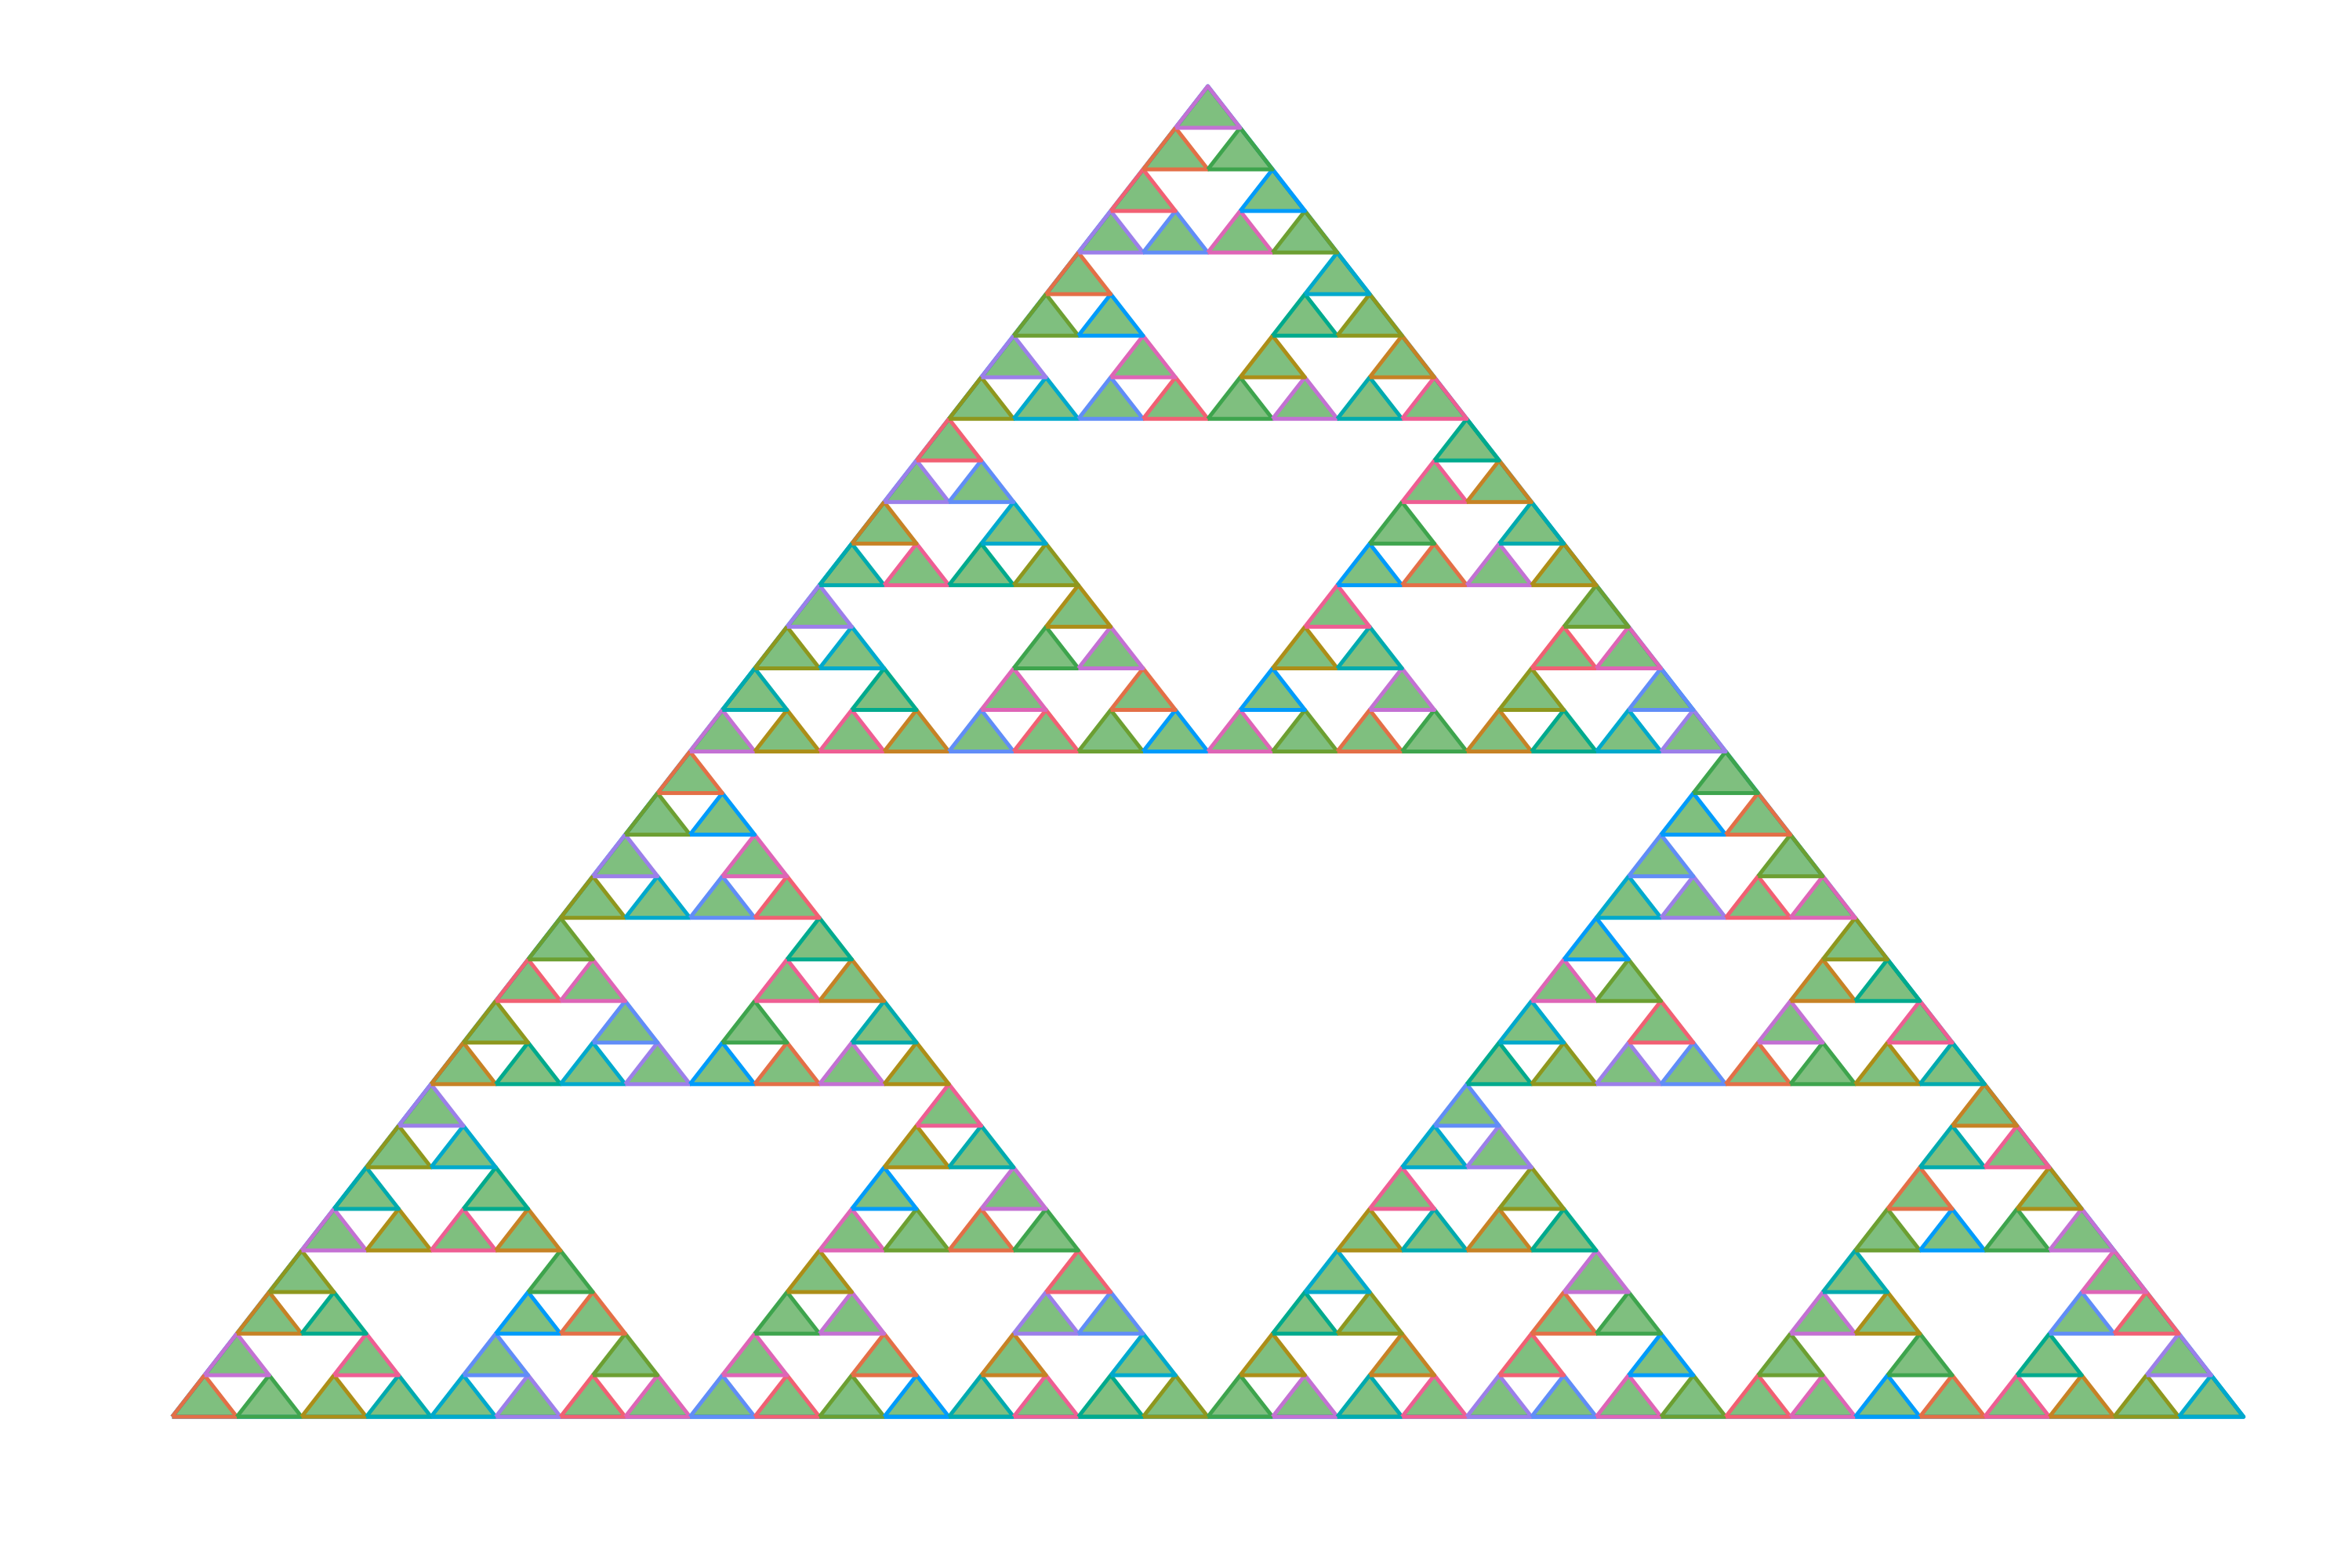
\includegraphics[scale = 0.027]{/Q3/SPT-O5}
        \label{fig:3.1.3}
        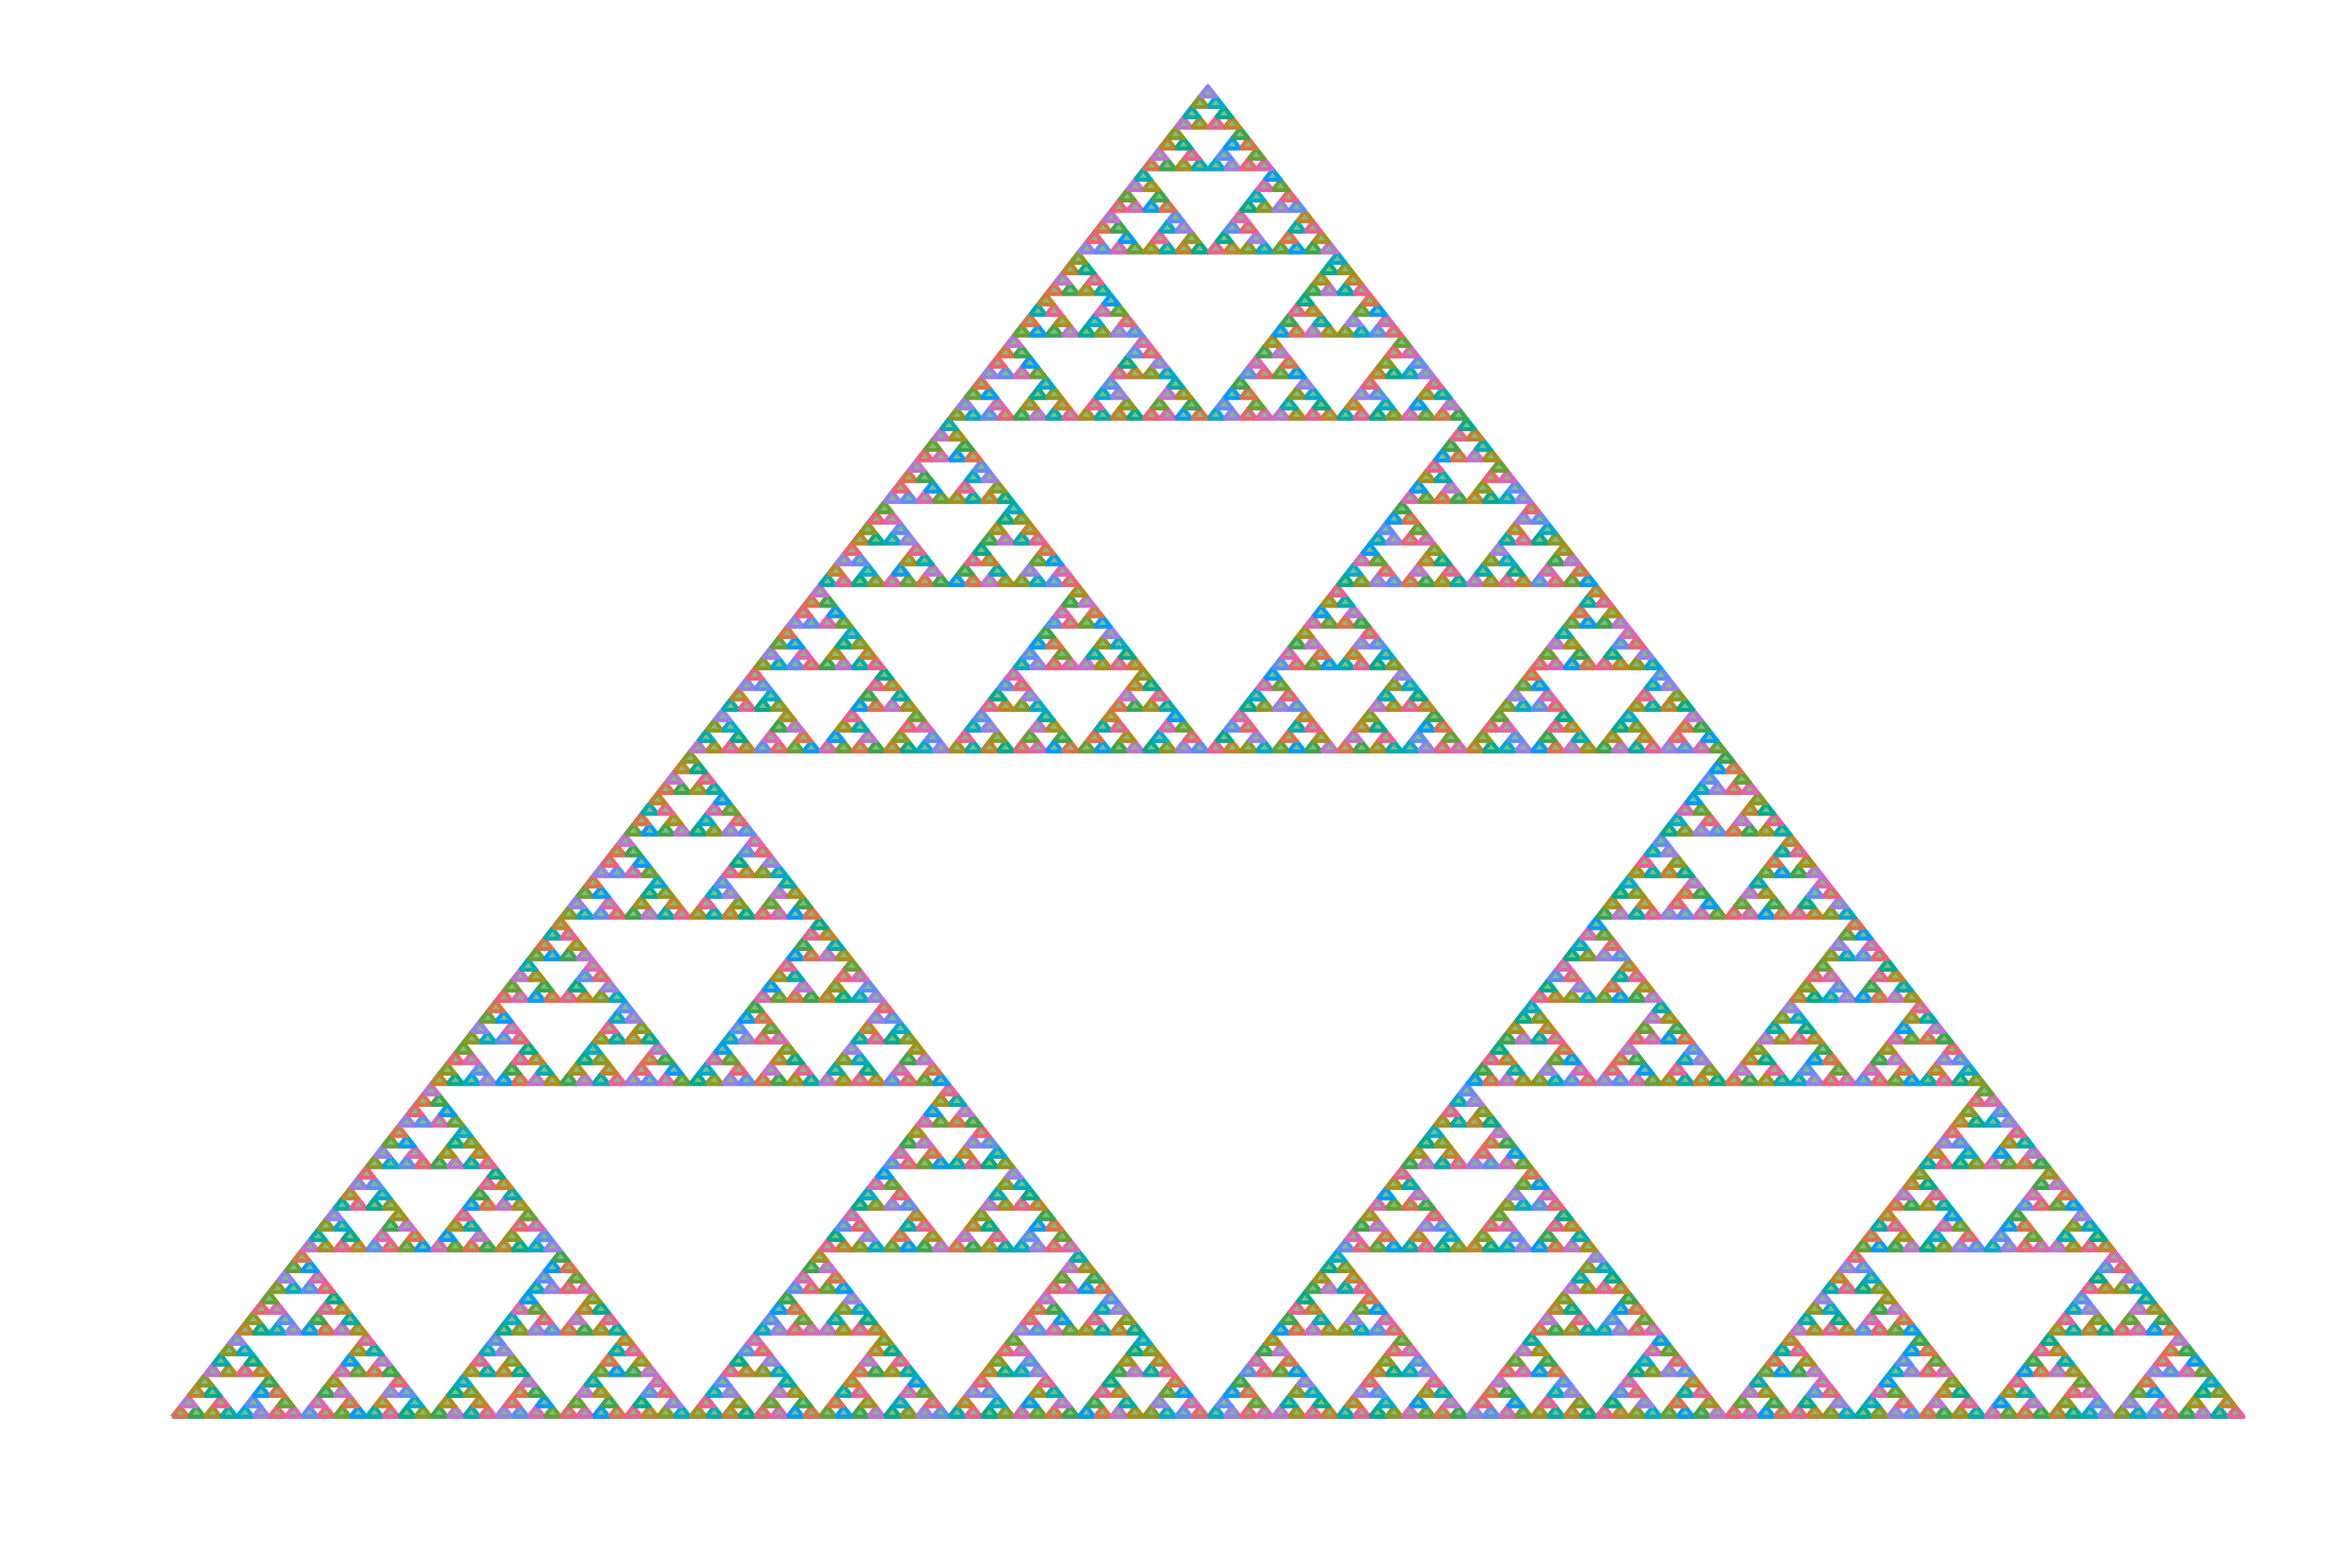
\includegraphics[scale = 0.027]{/Q3/SPT-O7}
        \label{fig:3.1.3}
        \caption{The Sierpinski triangle fractal. The figures belong to the 1st, 3th, 5th, and 7th stages, respectively.}
    \end{figure}
    \section*{Problem 4}
    \textbf{Basic description:}

    There we want to simulate the Sierpinski triangle using random computational methods.
    In that case, we will choose some random points on the surface.
    Then we will transit the points with three transmission functions.
    For each point, we will do this operation P times.
    We must note that in each step,
    we will choose a random function for applying.
    Our functions are as follows:

    $f_{1} = [x, y] \div 2$

    $f_{2} = [x, y] \div 2 + [1, 0]$

    $f_{3} = [x, y] \div 2 + [0, 1]$

    \begin{figure}[!htb]
        \centering
        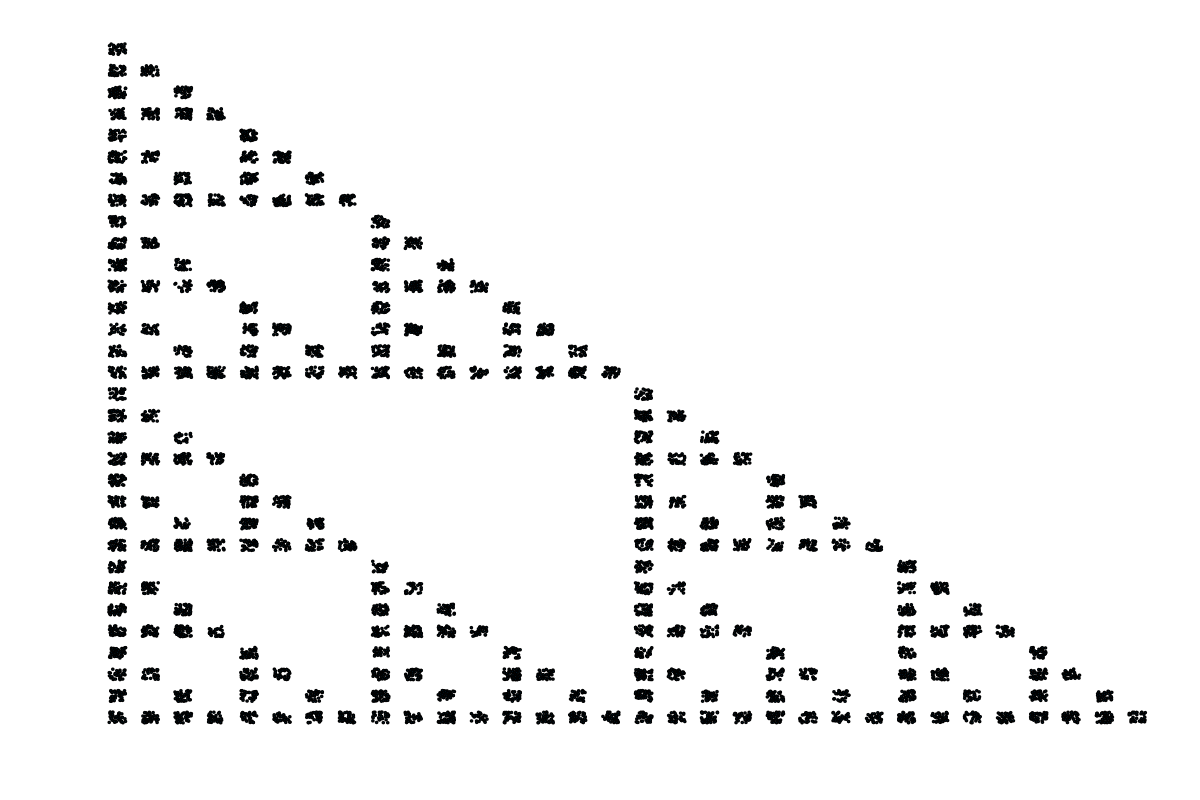
\includegraphics[scale = 0.1]{/Q4/RSPTp5num10000}
        \label{fig:4.1.1}
        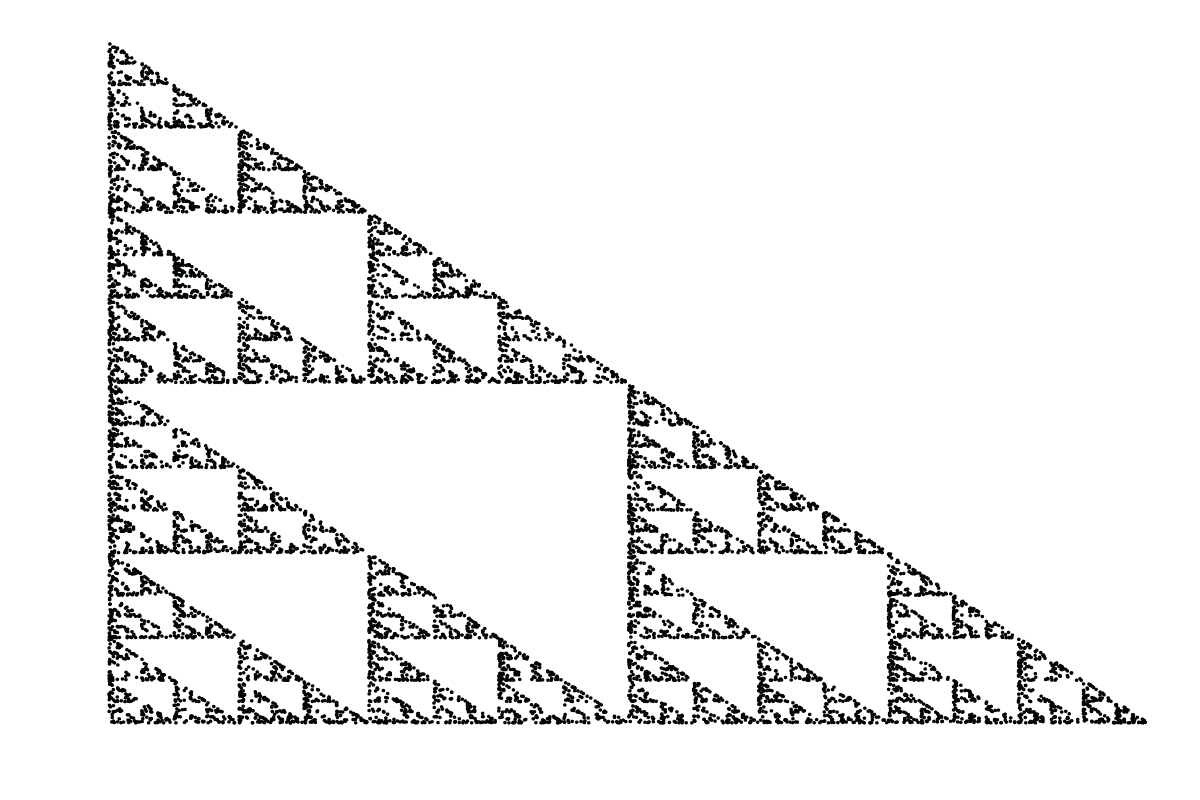
\includegraphics[scale = 0.1]{/Q4/RSPTp500num10000}
        \label{fig:4.1.2}
        \caption{The of deployed points is 10000 and P is 5 and 500 respectively.}
    \end{figure}
    \begin{figure}[!htb]
        \centering
        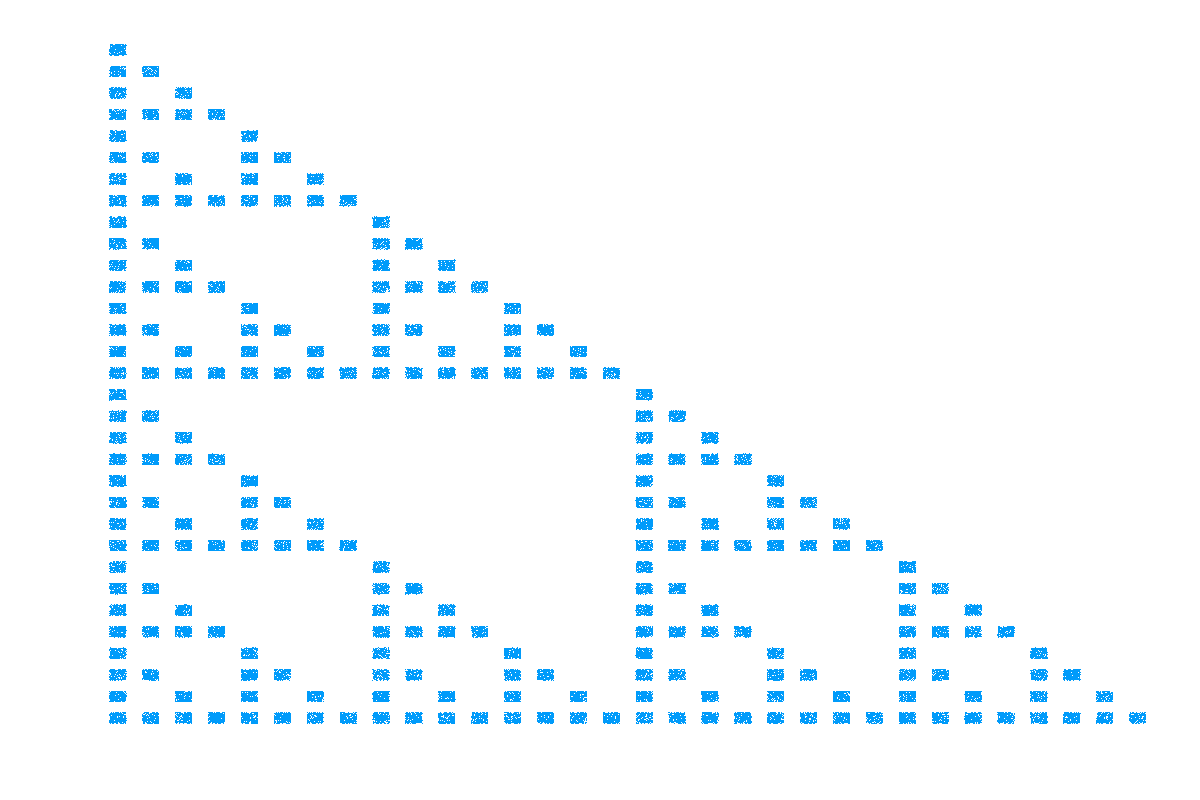
\includegraphics[scale = 0.1]{/Q4/RSPTp5num100000}
        \label{fig:4.2.1}
        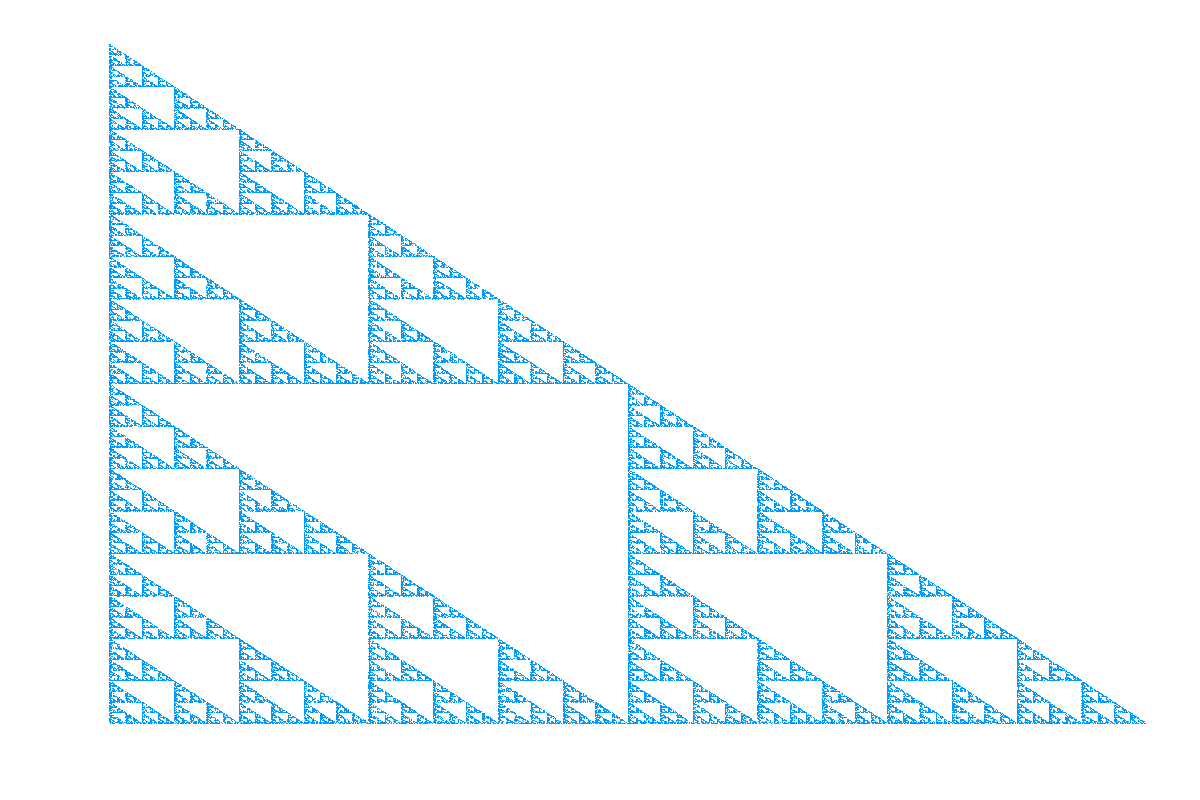
\includegraphics[scale = 0.1]{/Q4/RSPTp500num100000}
        \label{fig:4.2.2}
        \caption{The of deployed points is 100000 and P is 5 and 500 respectively.}
    \end{figure}
    \section*{Problem 5}
    \textbf{Basic description:}

    There we want to simulate the Sierpinski triangle using the Khayyam-Pascal's triangle.
    We know that if we separate the odd and even numbers of the Khayyam-Pascal's triangle we have the Sierpinski triangle.
    If we continue the Khayyam-Pascal's triangle up to $2^n$ ser stage our Sierpinski triangle will complete up to the nth stage.
    
    here is the results:

    \begin{figure}[!htb]
        \centering
        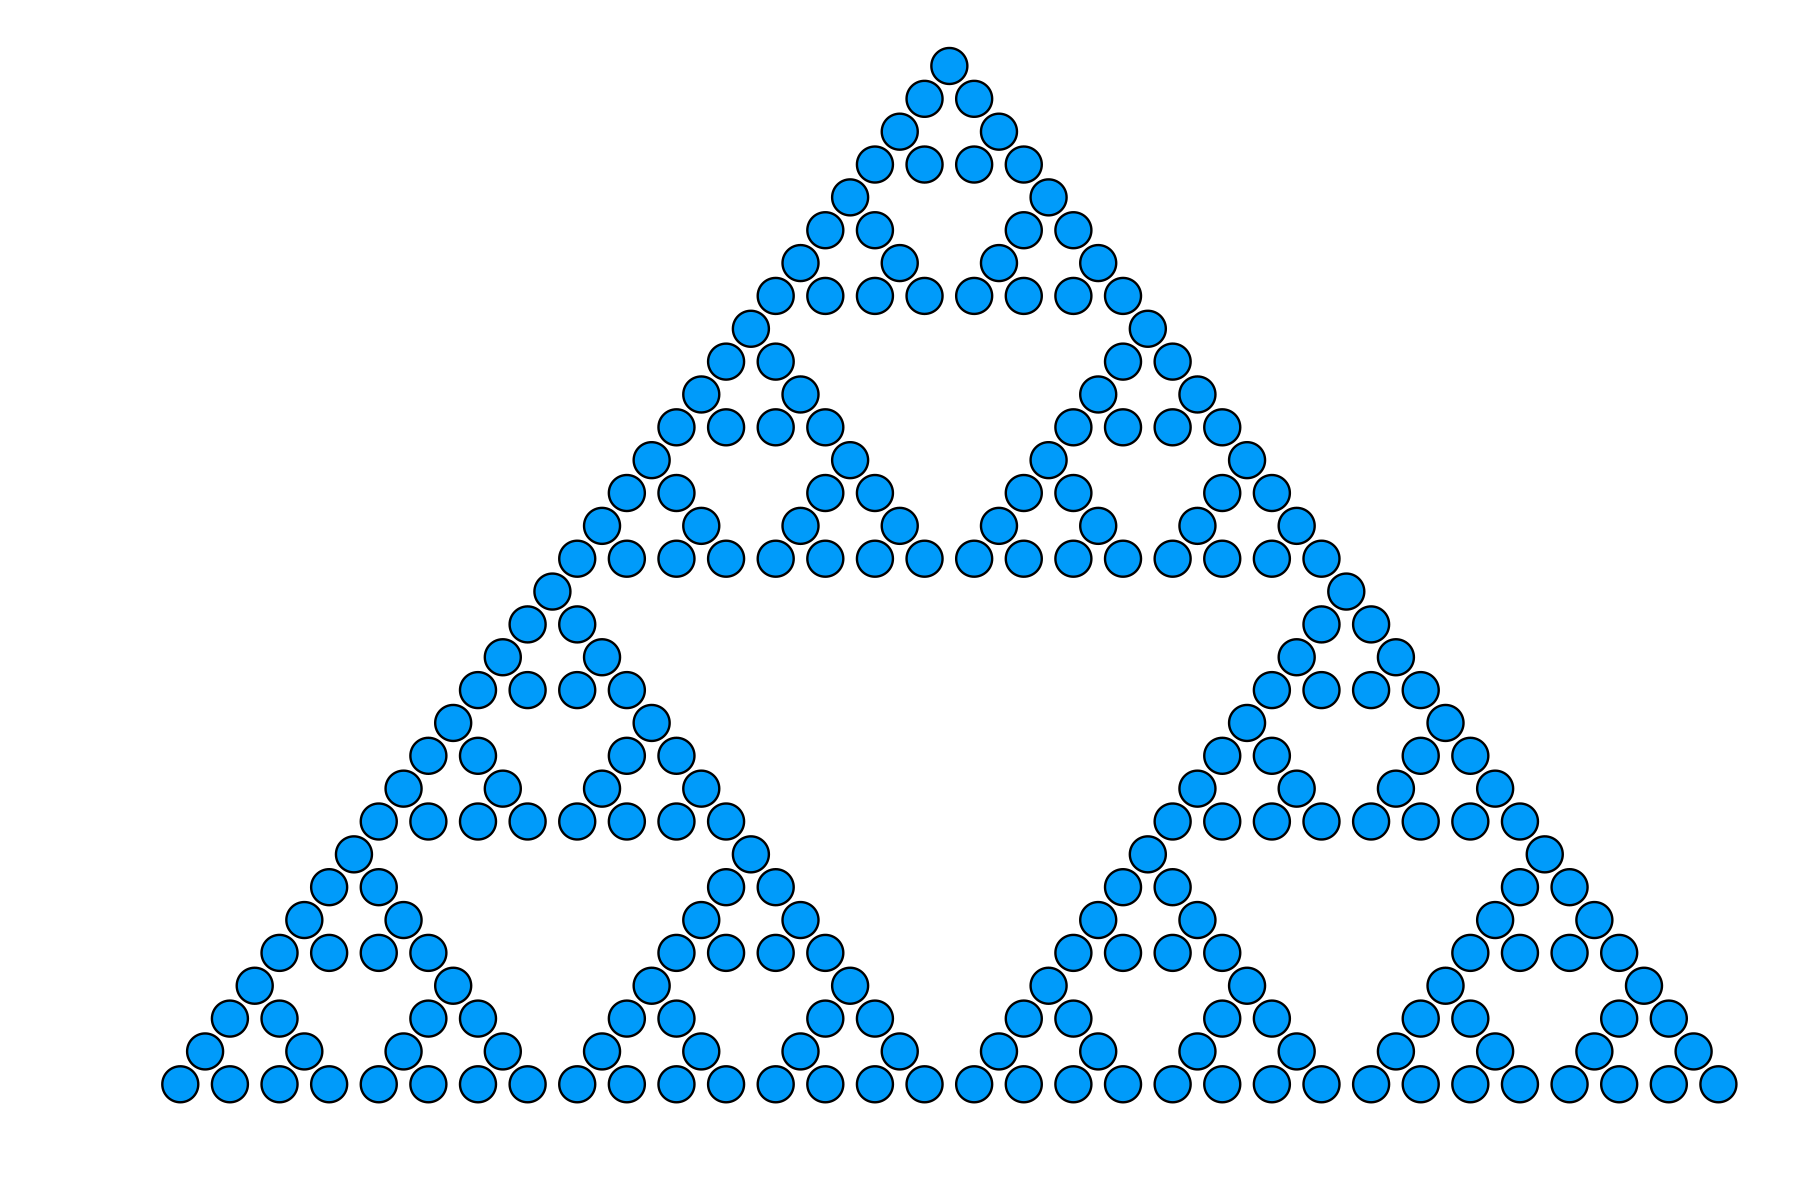
\includegraphics[scale = 0.05]{/Q5/SPTKP-O1}
        \label{fig:5.1.1}
        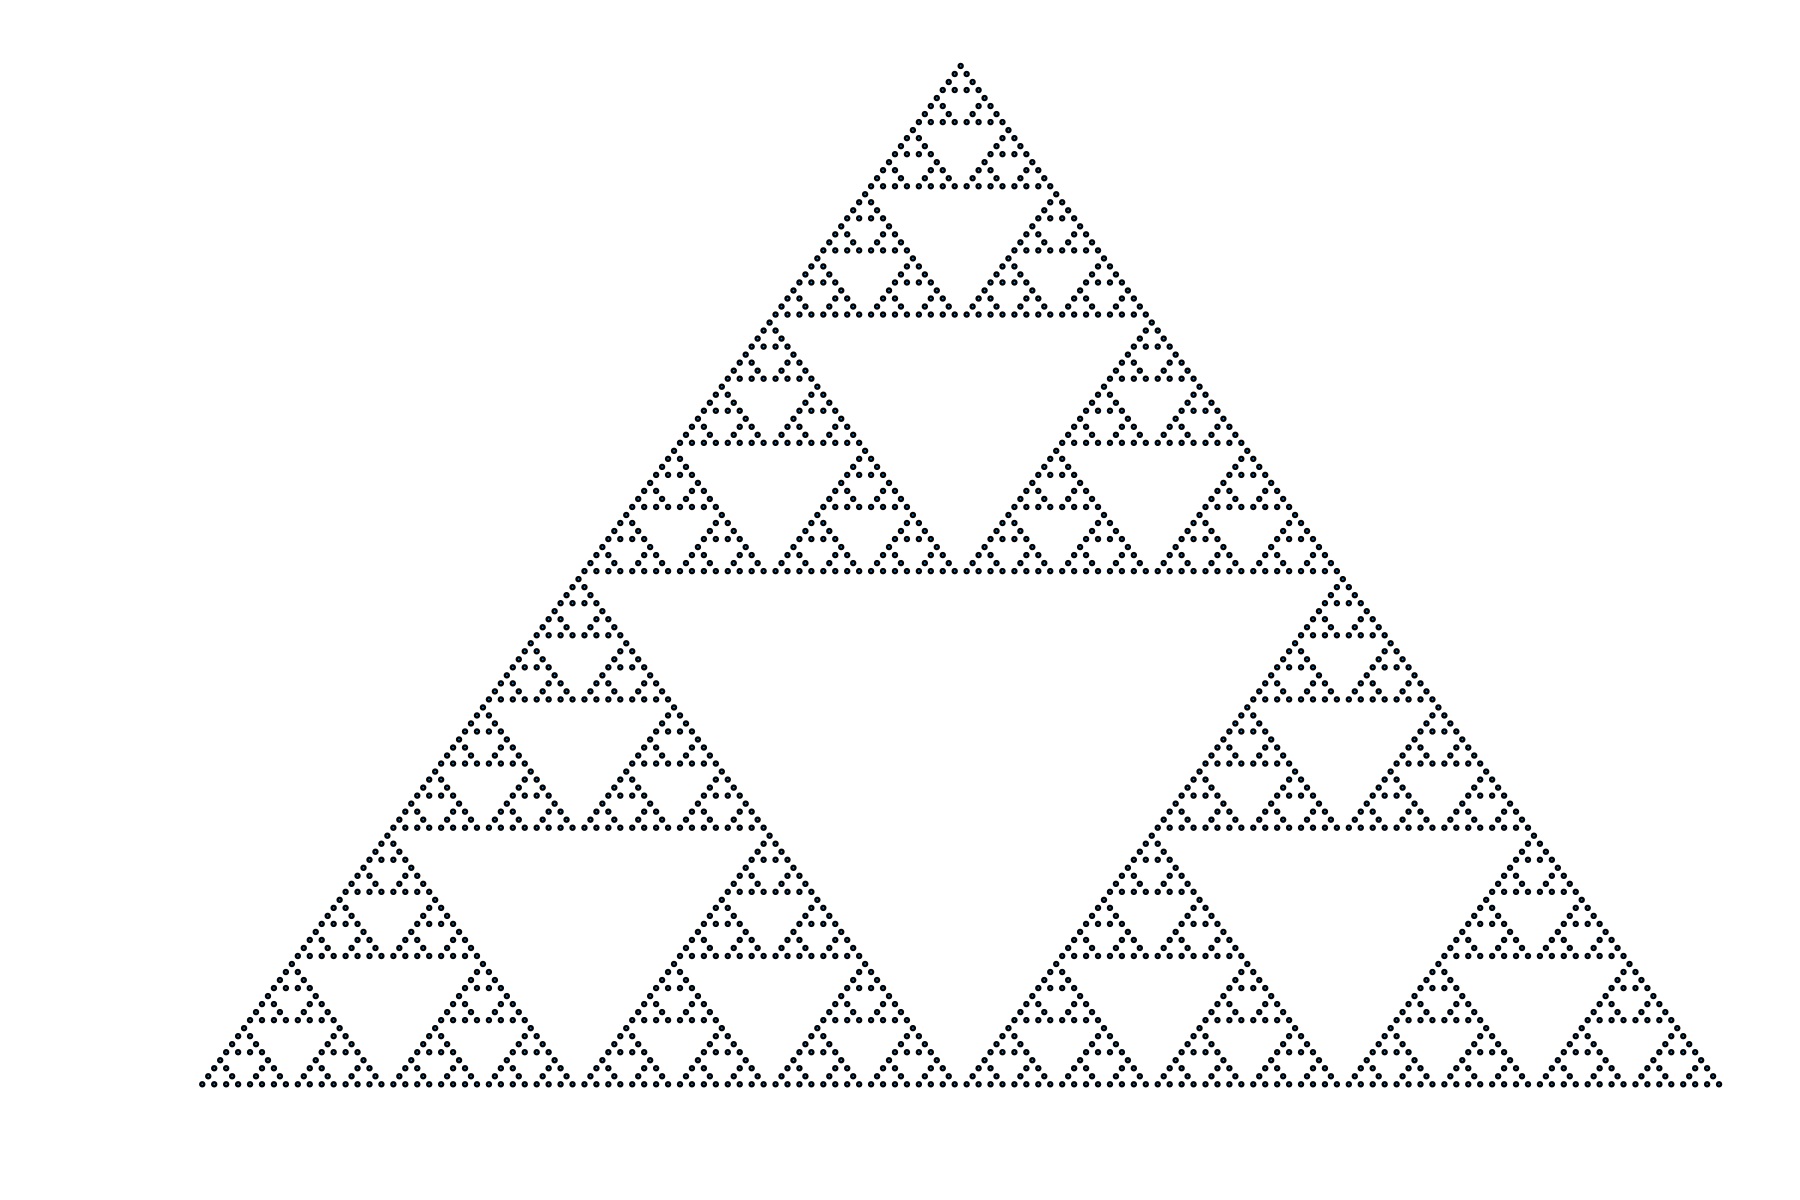
\includegraphics[scale = 0.05]{/Q5/SPTKP-O2}
        \label{fig:5.1.2}
        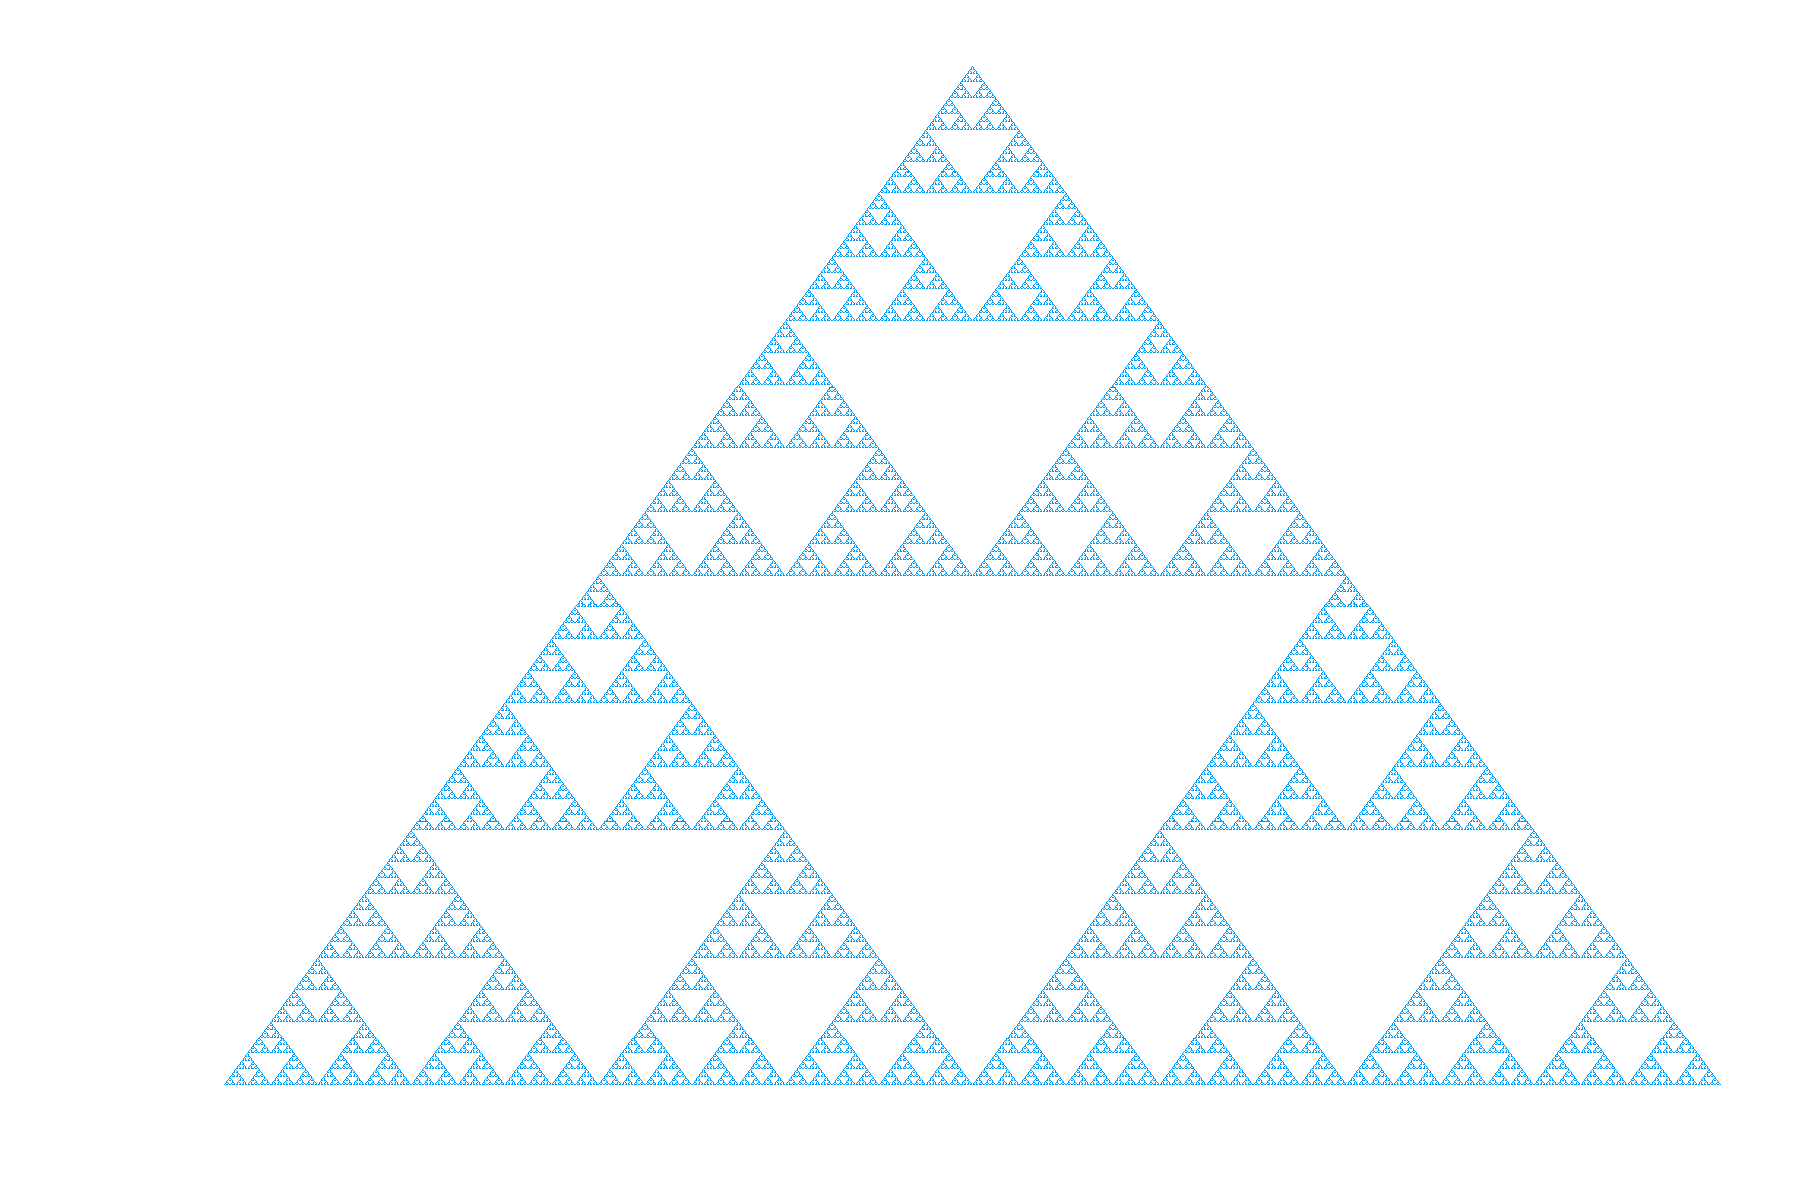
\includegraphics[scale = 0.05]{/Q5/SPTKP-O3}
        \label{fig:5.1.3}
        \caption{The Sierpinski triangle fractal. The $n$ equals 1, 2, and 3, respectively.}
    \end{figure}
    \section*{Problem 6}
    \textbf{Basic description:}

    There we want to simulate the Barnsley fern fractal using random computational methods.
    The method is the same as the random method for creating the Sierpinski triangle.
    Our functions are as follows:

    $f_{1}(x, y)=\left[\begin{array}{cc}0.00 & 0.00 \\ 0.00 & 0.16\end{array}\right]\left[\begin{array}{l}x \\ y\end{array}\right]$
    
    $f_{2}(x, y)=\left[\begin{array}{cc}0.85 & 0.04 \\ -0.04 & 0.85\end{array}\right]\left[\begin{array}{l}x \\ y\end{array}\right]+\left[\begin{array}{l}0.00 \\ 1.60\end{array}\right]$
    
    $f_{3}(x, y)=\left[\begin{array}{cc}0.20 & -0.26 \\ 0.23 & 0.22\end{array}\right]\left[\begin{array}{l}x \\ y\end{array}\right]+\left[\begin{array}{l}0.00 \\ 1.60\end{array}\right]$
    
    $f_{4}(x, y)=\left[\begin{array}{cc}-0.15 & 0.28 \\ 0.26 & 0.24\end{array}\right]\left[\begin{array}{l}x \\ y\end{array}\right]+\left[\begin{array}{l}0.00 \\ 0.44\end{array}\right]$

    \begin{figure}[!htb]
        \centering
        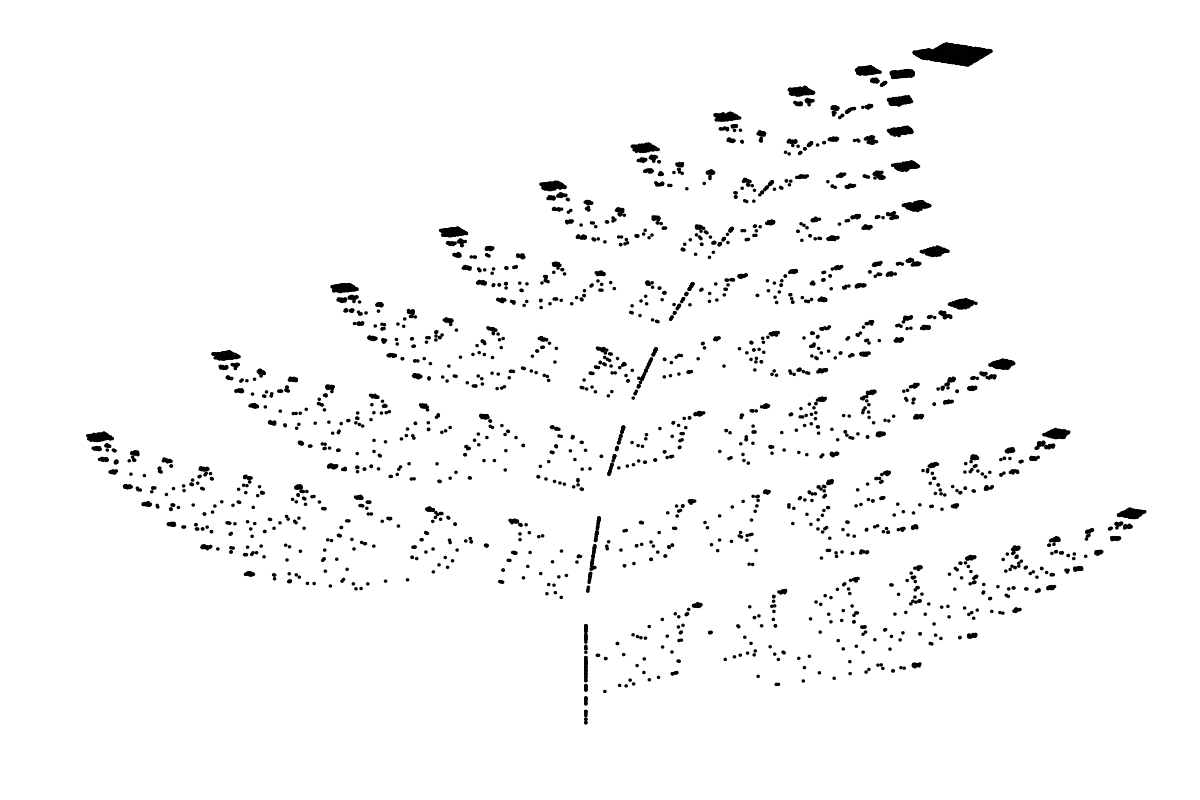
\includegraphics[scale = 0.1]{/Q6/RandomBarnsleyFern-p10num10000}
        \label{fig:6.1.1}
        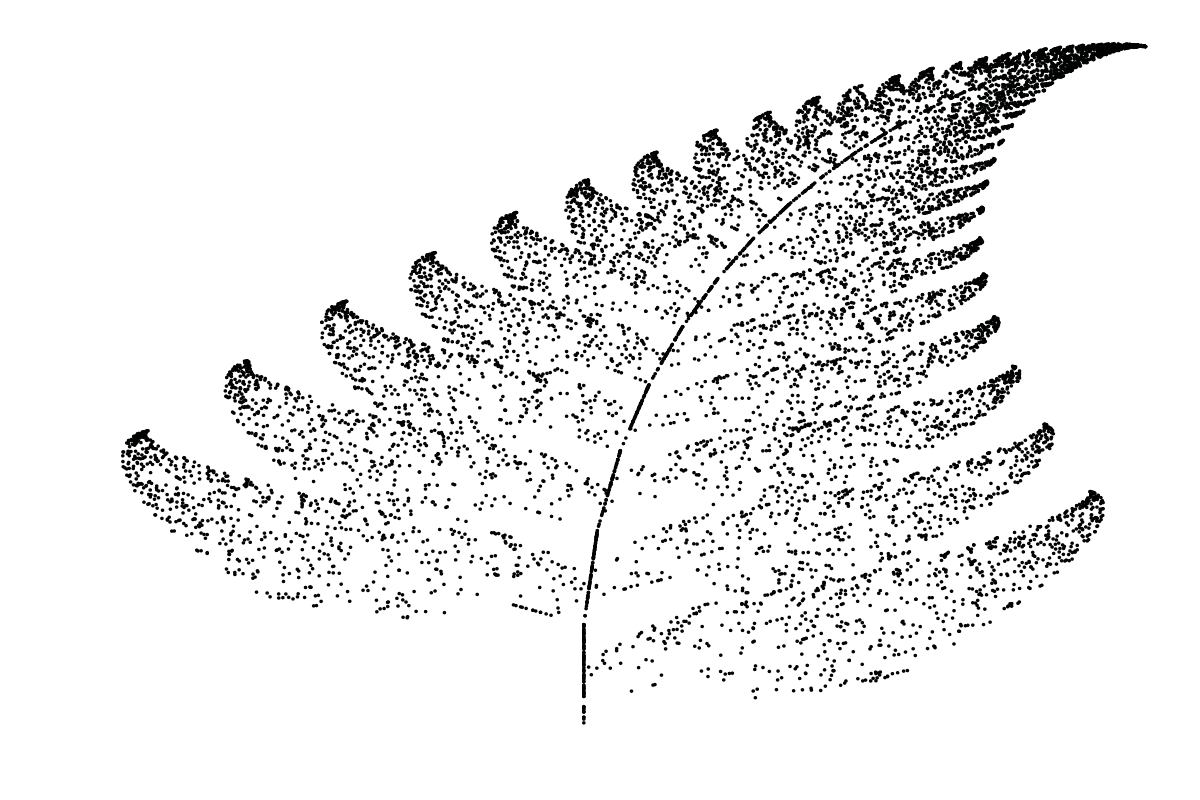
\includegraphics[scale = 0.1]{/Q6/RandomBarnsleyFern-p100num10000}
        \label{fig:6.1.2}
        \caption{The of deployed points is 10000 and P is 10 and 100 respectively.}
    \end{figure}
    \begin{figure}[!htb]
        \centering
        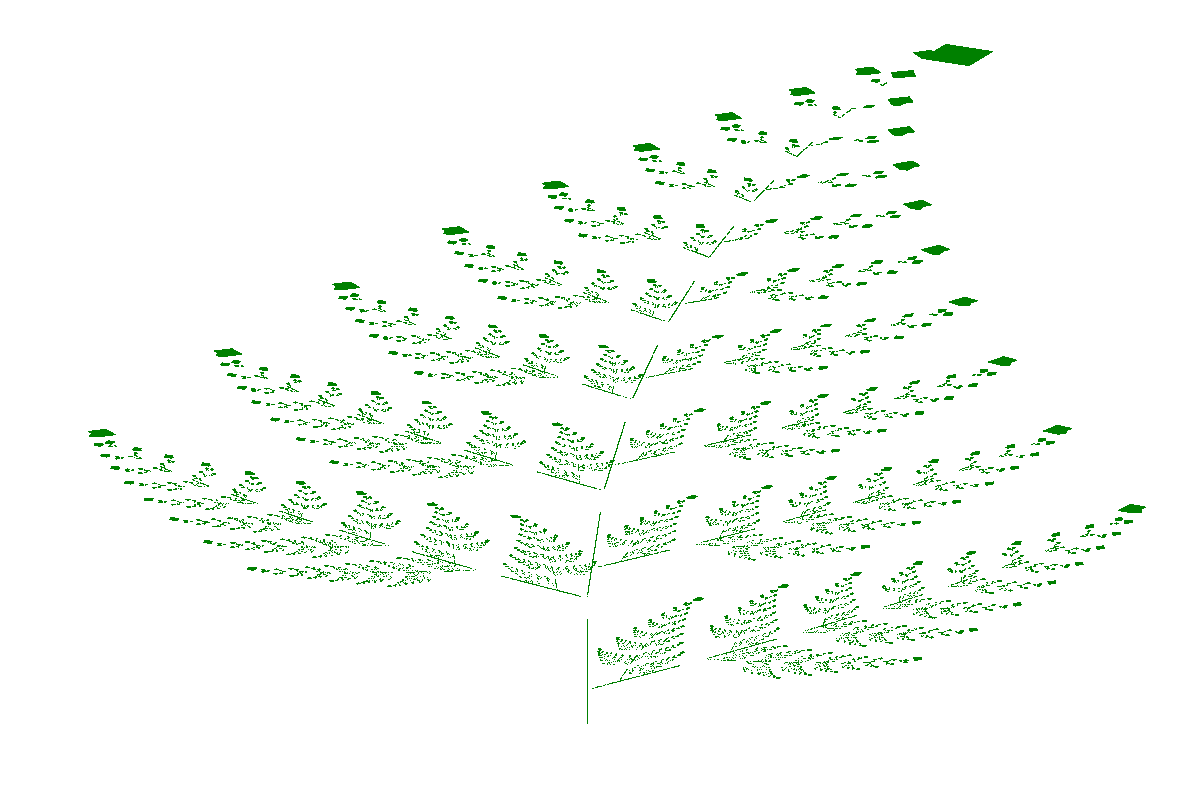
\includegraphics[scale = 0.1]{/Q6/RandomBarnsleyFern-p10num1000000}
        \label{fig:6.2.1}
        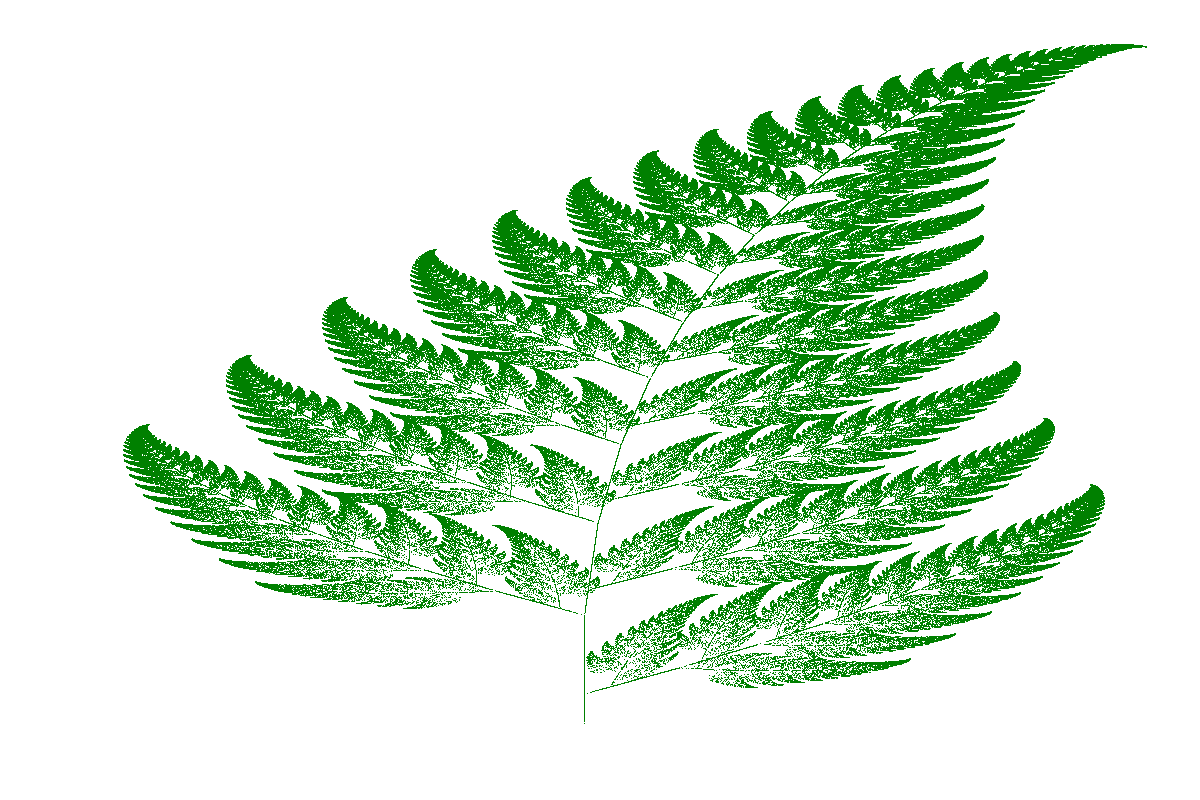
\includegraphics[scale = 0.1]{/Q6/RandomBarnsleyFern-p100num1000000}
        \label{fig:6.2.2}
        \caption{The of deployed points is 1000000 and P is 10 and 100 respectively.}
    \end{figure}
\end{document}